\documentclass[tikz,border=4pt]{standalone}
\usepackage{amsmath}
\begin{document}
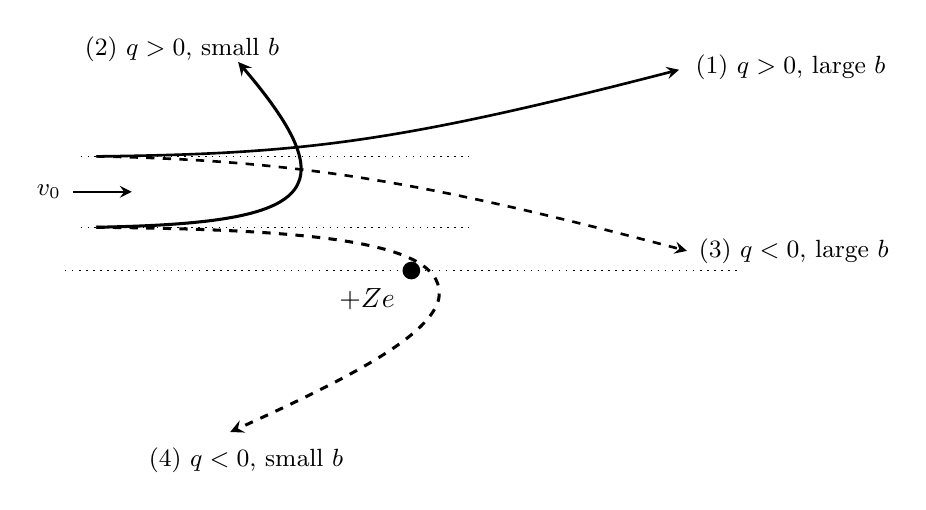
\begin{tikzpicture}[>=stealth, thick, scale=1.0]
  % Nucleus at origin (0,0)
  \draw[dotted, line width=0.55pt] (-4.4, 0) -- (4.2, 0);
  \fill (0, 0) circle (3.2pt);
  \node[below left] at (-0.08, -0.10) {$+Ze$};

  % Asymptotic incoming lines for large b (y = 1.45) and small b (y = 0.55)
  \draw[dotted, line width=0.5pt] (-4.2, 1.45) -- (0.8, 1.45);
  \draw[dotted, line width=0.5pt] (-4.2, 0.55) -- (0.8, 0.55);

  % Exact hyperbolic trajectories:
  % Repulsive (q > 0): bends upward (away from nucleus)
  % Large b (solid): slight upward deflection
  \draw[->, line width=0.95pt] (-4.0, 1.45) .. controls (-1.4, 1.48) and (-0.2, 1.62) .. (3.4, 2.55);
  \node[right, font=\small] at (3.48, 2.58) {(1) $q > 0$, large $b$};

  % Small b (solid thick): strong upward/backward deflection
  \draw[->, line width=1.1pt] (-4.0, 0.55) .. controls (-1.3, 0.60) and (-0.75, 0.95) .. (-2.2, 2.65);
  \node[above left, font=\small] at (-1.55, 2.52) {(2) $q > 0$, small $b$};

  % Attractive (q < 0): bends downward (toward nucleus)
  % Large b (dashed): slight downward deflection
  \draw[->, line width=0.95pt, dashed] (-4.0, 1.45) .. controls (-1.4, 1.40) and (0.2, 1.12) .. (3.5, 0.25);
  \node[right, font=\small] at (3.52, 0.25) {(3) $q < 0$, large $b$};

  % Small b (dashed thick): strong downward deflection swinging past nucleus
  \draw[->, line width=1.1pt, dashed] (-4.0, 0.55) .. controls (-1.1, 0.52) and (0.45, 0.35) .. (0.35, -0.35) .. controls (0.25, -0.82) and (-0.75, -1.35) .. (-2.3, -2.05);
  \node[below, font=\small] at (-2.1, -2.12) {(4) $q < 0$, small $b$};

  % Incoming direction label
  \draw[->, line width=0.9pt] (-4.3, 1.00) -- (-3.55, 1.00);
  \node[left, font=\small] at (-4.32, 1.00) {$v_0$};
\end{tikzpicture}
\end{document}
